% Adjusting chapter title format for regular (numbered) chapters
\titleformat{\chapter}[display]
  {\normalfont\huge\bfseries\centering}{\chaptertitlename\ \thechapter}{20pt}{\Huge}

% Using similar styling for unnumbered chapters but without "Chapter" prefix
\titleformat{name=\chapter,numberless}
  {\normalfont\huge\bfseries\centering}{}{0pt}{\Huge}

\titlespacing*{\chapter}{0pt}{50pt}{40pt} % Adjust vertical spacing before and after the title

\chapter{Introduction} % Ensures chapter numbering starts correctly

\section{Overview} % This will now be Section 1.1, not 0.1

Deep Neural Networks (DNNs) are increasingly being used in diverse applications due to their ability to match or exceed human-level performance. The availability of large datasets, fast computing methods, and their high performance has paved the way for DNNs in safety-critical applications such as autonomous driving, medical diagnosis, and security. The safety-critical nature of such applications makes it imperative to adequately test these DNNs before deployment. However, unlike traditional software, DNNs do not have a clear control-flow structure. They learn their decision policy through training on large datasets, adjusting parameters gradually using various methods to achieve the desired accuracy. Consequently, traditional software testing methods like functional coverage and branch coverage cannot be applied to DNNs, thus challenging their use in safety-critical applications.

Recent work, discussed in Chapter II, has focused on developing testing frameworks for DNNs. These methods suffer from certain limitations, as discussed in the challenges section. In our work, we aim to overcome these limitations and build a fast, scalable, efficient, and generalizable testing framework for deep neural networks.

In this section of the thesis, the background and motivation, research questions, contributions, and organization of the thesis are presented.

\subsection{Background and Motivation}

In recent years, DNNs have made remarkable progress in achieving human-level performance. With the broader deployment of DNNs in various safety-critical systems like autonomous vehicles, healthcare, and avionics, concerns over their safety and trustworthiness have been raised, particularly highlighted by incidents involving self-driving cars.

An important requirement for DNNs is robustness against input perturbations. DNNs have been shown to lack robustness due to their susceptibility to adversarial examples, where small modifications to an input, sometimes imperceptible to humans, can make the network unstable.

This thesis examines existing testing methods for DNNs, opportunities for improvement, and the need for a fast, scalable, generalizable end-to-end testing method.

Coverage criteria for traditional software programs, such as code coverage and branch coverage, ensure that all parts of the logic in the program have been tested by at least one test input and all conditions have been tested to independently affect the entailing decisions. Similarly, any coverage criterion for DNNs must ensure that all parts of the internal decision-making structure of the DNN have been exercised by at least one test input.

Generating or selecting test inputs in a guided manner usually has two major goals: maximizing the number of uncovered faults and maximizing the coverage.

Testing DNNs for correctness involves verifying behaviors against a ground truth or oracle. The traditional approach of collecting and manually labeling real-world data is labor-intensive. Another method compares outputs across multiple DNNs for the same task, identifying discrepancies as corner cases. However, this can misclassify inputs if all models agree, due to shared biases or errors. This comparative approach is further limited to tasks with multiple reliable models, which may not always be available, especially in innovative or specialized applications.

\begin{figure*}[h]
	\centering
	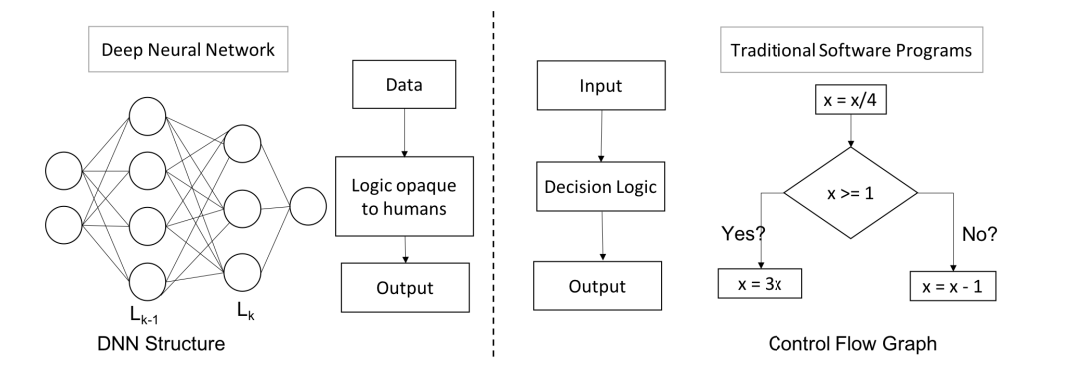
\includegraphics[width=0.8\textwidth]{fig1.png}
	\caption{The internal logic of a deep neural network is opaque to humans, unlike the well-laid-out decision logic of traditional software programs \cite{Intro_1}}
	\label{fig:1}
\end{figure*}

\begin{figure*}[h]
	\centering
	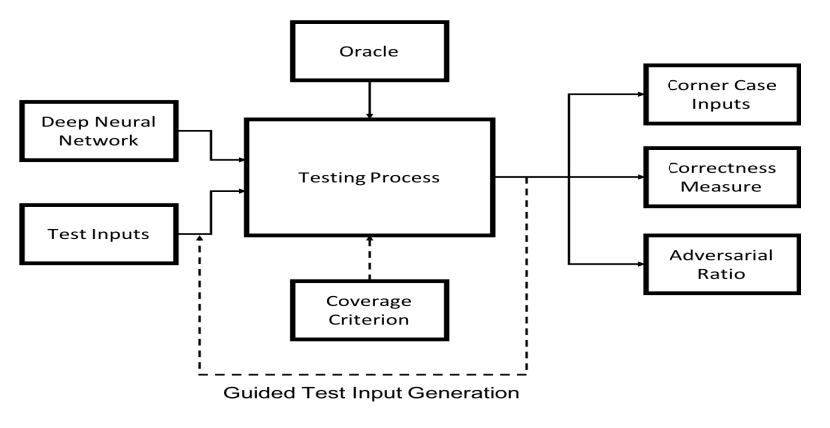
\includegraphics[width=0.8\textwidth]{fig2.png}
	\caption{A high-level representation of most existing DNN testing methods \cite{Intro_1}}
	\label{fig:2}
\end{figure*}

\subsection{Challenges of Deep Learning Models}

The growing use of DNNs in safety-critical applications necessitates adequate testing to detect and correct any incorrect behavior for corner case inputs before deployment. DNNs lack an explicit control-flow structure, making it impossible to apply traditional software testing criteria such as code coverage.

\begin{itemize}
	\item The input space is extremely large, making unguided simulations highly unlikely to find erroneous behavior.
\end{itemize}

\subsection{Challenges in Testing of Deep Learning Models}

Unlike traditional software, DNNs do not have a clear control-flow structure. They learn their decision policy through training on a large dataset, adjusting parameters gradually using several methods to achieve desired accuracy. Consequently, traditional software testing methods like functional coverage, branch coverage, etc., cannot be applied to DNNs, thereby challenging their use in safety-critical applications. Traditional software testing methods fail when applied to DNNs because the code for deep neural networks holds no information about the internal decision-making logic of a DNN.

DNN testing techniques aim to discover bugs by finding counterexamples that challenge the system's correctness or to establish confidence by rigorously evaluating the system with numerous test cases. These testing techniques are computationally less expensive and therefore can work with state-of-the-art DNNs. However, DL testing has some limitations:
\begin{itemize}
    \item Standards available in the industry but \textbf{Lack of Logical Structure} and \textbf{System Specification}
    \item Heavily dependent on manual collections of test data under different conditions, which become expensive as the number of test conditions increases
    \item Existing coverage criteria are not detailed enough to notice subtle behaviors exhibited by DL systems
\end{itemize}

\subsection{Problem Statement}

Deep learning models are being more widely used in various applications, yet their reliability in practical applications remains a challenge.

\subsection{Research Goal}

This thesis aims to develop a systematic framework for evaluating local and global robustness in deep learning models. The goal is to provide a comprehensive error summary to improve model design and training, ensuring their reliability for real-world applications.

\subsection{Research Questions}\hypertarget{researchquestions}{}
\begin{itemize}
	\item How can we sample inputs efficiently?
	\item How can we design a comprehensive framework to test system robustness?
    \item How can we systematically evaluate the robustness both at local (property-specific) and global (overall system) levels within the framework?
    \item How can error summarization be employed to quantify the impacts on model robustness?
\end{itemize}

\subsection{Thesis Contributions}\hypertarget{contributions}{}

This research makes the following key contributions to the field of deep learning robustness evaluation:
\begin{itemize}
    \item We design an \textbf{end-to-end pipeline} for evaluating the correctness of the system.
    \item We propose a \textbf{conceptual framework} that quantifies both local and global correctness, with a formalized Bayesian probabilistic approach to verify system robustness.
    \item A novel \textbf{error summarization} approach which allows better identification of model weaknesses related to class and property.
    \item We perform all our \textbf{experiments} using publicly available deep learning models and the MNIST dataset.
\end{itemize}

\subsection{Organization of the Thesis}\hypertarget{organization of thesis}{}
The remainder of the thesis is organized as follows: related studies are presented in Chapter \ref{chp:2}. The system model and proposed methodology are demonstrated in Chapter \ref{chp:3}. Chapter \ref{chp:4} describes the simulation results of our proposed schemes. Finally, the findings of this work along with future directions are presented in Chapter \ref{chp:6}.

\clearpage
